\begin{figure}[H]
    \centering
    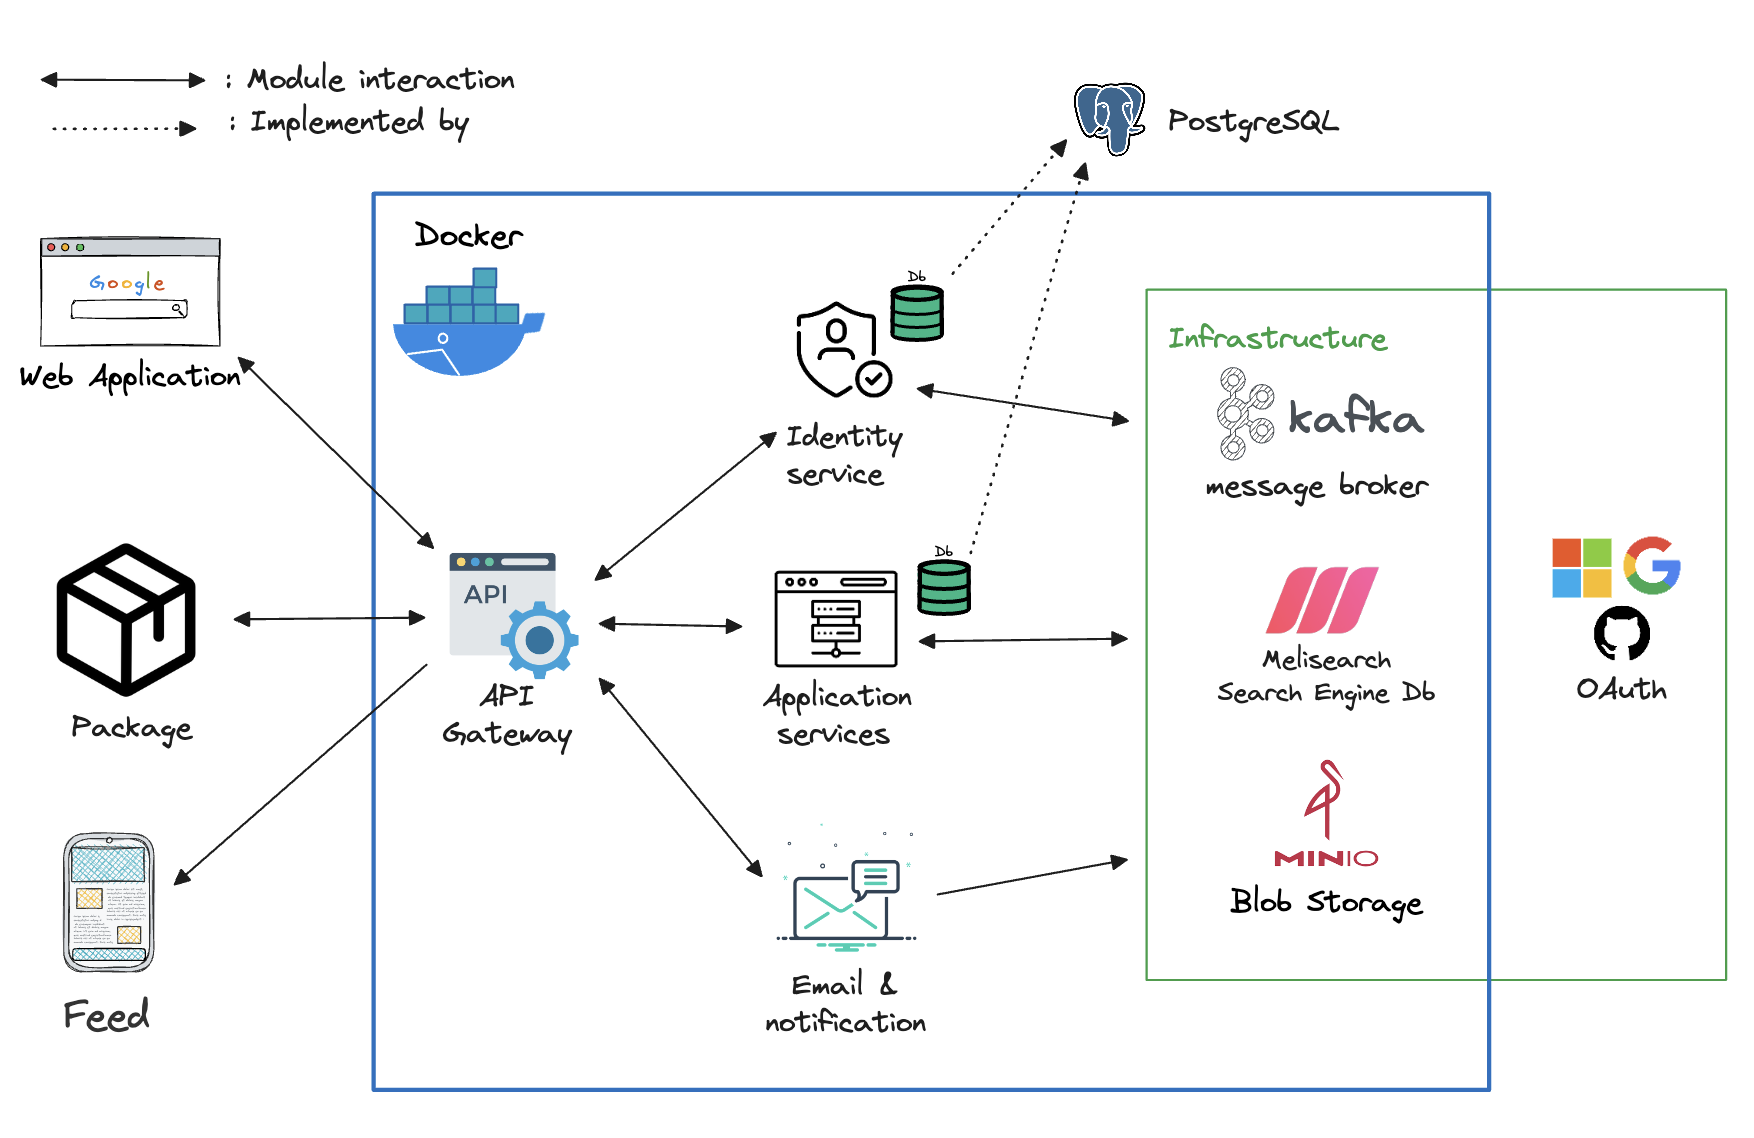
\includegraphics[width=\linewidth]{Images/arch.png}
    \vspace{1em}
    \caption{System Architecture}
    \label{fig:sow}
\end{figure}
\vspace{0.5cm}
Based on the requirements set by stakeholders and after studying the existing
system, the team proposes the design and implementation of a Weather Data Platform. Figure
\ref{fig:sow} illustrates the implementation of the system.
\newpage

\subsection{Microservices}

In essence, a microservices architecture decomposes a large software application
into a collection of smaller, self-contained services. Each service plays a
specific role and owns a well-defined business capability. These services are
loosely coupled, meaning they interact through well-designed APIs and operate independently.

Microservices architectures offer a compelling approach to building software. By
decomposing large applications into smaller, independent services, they unlock
agility, maintainability, and fault isolation.  Each service owns a specific
business function and interacts with others through well-defined APIs. This
allows for faster development cycles, easier maintenance of individual services,
and the freedom to choose the best technology for each job.

However, this power comes with a price. Managing a distributed system with
numerous services inherently increases complexity compared to a monolithic
application. Communication between services adds overhead to the system's
performance. Perhaps the most significant challenge lies in ensuring data
consistency across these independent services, requiring meticulous design and
implementation.  Carefully considering these trade-offs is crucial before
embarking on a microservices journey.

While microservices boast impressive agility and maintainability, adopting this
architecture isn't without its complexities.  Managing a distributed system with
numerous services inherently increases complexity compared to a monolithic
application.  Furthermore, communication between these services adds overhead to
the system's performance.  Perhaps the most significant challenge lies in
ensuring data consistency across these independent services, requiring
meticulous design and implementation.

\subsection{Clean Architecture}

Microservices and Clean Architecture can complement each other to create a
modular, maintainable, and scalable system. Microservices architecture promotes
the development of small, independent services that can be deployed, scaled, and
updated independently. Each microservice encapsulates a specific business
capability or domain, reducing the overall complexity of the system.

Clean Architecture, on the other hand, advocates for a layered approach to
software design, promoting separation of concerns and decoupling of components.
By adhering to the principles of Clean Architecture within each microservice,
developers can achieve a high degree of modularity, testability, and
maintainability.

Clean Architecture separates the system into distinct layers, each with specific
responsibilities. The Shared Kernel acts as the core, housing reusable
components that benefit all layers. The Domain layer sits at the heart of the
application, defining core entities and their behaviors. A common base class
promotes code maintainability within this layer. The Application layer
orchestrates request routing and establishes project-wide contracts for
implementation in other layers. Clean Architecture emphasizes the testability of
each layer through unit tests. Frameworks like xUnit simplify unit test
creation. 

The Infrastructure layer provides supporting services for the application.
Cross-cutting concerns like logging reside here. User registration,
authentication, and authorization functionalities are handled by the Identity
layer. Persistence takes care of data access using patterns like repositories
and Unit of Work. The Web Framework layer manages configurations for the web
application, while the Web API layer delivers functionality to the user.
Finally, plugins bridge the gap between monolithic and microservices
architectures by promoting modularity.

